%%%%%%%%%%%%%%%%%%%%%%%%%%%%%%%%%%%%%%%%%%%%%%%%%%%%%%%
%                   File: OSAmeetings.tex             %
%                  Date: 20 September 2021            %
%                                                     %
%     For preparing LaTeX manuscripts for submission  %
%       submission to Optica meetings and conferences %
%                                                     %
%       (c) 2021 Optica                               %
%%%%%%%%%%%%%%%%%%%%%%%%%%%%%%%%%%%%%%%%%%%%%%%%%%%%%%%

\documentclass[letterpaper,10pt]{article} 
%% if A4 paper needed, change letterpaper to A4

\usepackage{osameet3} %% use version 3 for proper copyright statement

%% standard packages and arguments should be modified as needed
\usepackage{amsmath,amssymb}
\usepackage[colorlinks=true,bookmarks=false,citecolor=blue,urlcolor=blue]{hyperref} %pdflatex
%\usepackage[breaklinks,colorlinks=true,bookmarks=false,citecolor=blue,urlcolor=blue]{hyperref} %latex w/dvipdf

\begin{document}

\title{Preparing a Manuscript for Submission to an Optica Meeting or Conference}

\author{Author name(s)}
\address{Author affiliation and full address}
\email{e-mail address}
%%Uncomment the following line to override copyright year from the default current year.
\copyrightyear{2022}


\begin{abstract}
\LaTeX{} users preparing manuscripts for Optica meetings or conferences
should use  the \texttt{osameet3.sty} style file and should observe these
guidelines to adhere to Optica requirements. Users of Bib\TeX{} may use the \texttt{osajnl.bst} style file, which is included in this distribution. Comments and questions should be directed to the Optica Conference Papers staff (tel: +1 202.416.6191,  e-mail: cstech@optica.org).
\end{abstract}

\section{Main Text}

\subsection{Required Elements}
All PDF submissions must contain the following items in order to be published:

\begin{enumerate}
\item Complete title
\item Complete listing of all authors and their affiliations
\item Self-contained abstract (indexers such as Google Scholar will not index papers that do not contain abstracts)
\item Appropriate copyright statement following the abstract. By default, the copyright statement will appear as \number\year \hskip.05in The Author(s). If needed, the default statement can be suppressed by use of the \verb+{abstract*}+ environment.
\item Permission and attribution for any trademarked or copyright images. Note that images of people or images owned or trademarked by other entities (including well-known logo's or cartoon characters for example) will also require official written permission.
\item Two-page limit unless designated otherwise on conference website
\end{enumerate}

\subsection{Typographical Style}
Margins and type size will be set by the Optica \LaTeX{}
commands for title, author names and addresses, abstract,
references, captions, and so on. The \texttt{osameet3.sty} package
references \texttt{mathptmx.sty} for Times text and math fonts.
Authors who require Computer Modern font may modify the style file
or, preferably, invoke the package \texttt{ae.sty} or similar for
optimum output with Computer Modern.

\subsection{Author Names and Affiliations}
Author names should be given in full with first initials spelled out to assist with indexing.
Affiliations should follow the format division, organization, and address---and complete postal information should be given.
Abbreviations should not be used. United States addresses should end
with ``, USA.''

\subsection{Abstract} The abstract
should be limited to no more than 35 words. It should be an
explicit summary of the paper that states the problem, the methods
used, and the major results and conclusions. If another publication author is referenced in the abstract, abbreviated information
(e.g., journal, volume number, first page, year) must be
given in the abstract itself, without a reference number. (The item referenced in the abstract should be the first
cited reference  in the body.)

\subsection{Notation}
\subsubsection{General Notation}
Notation must be
legible, clear, compact, and consistent with standard usage. In
general, acronyms should be defined at first use.


\subsubsection{Math Notation}
Equations should use standard \LaTeX{} or AMS\LaTeX{} commands (sample from Krishnan \textit{et al.} \cite{krishnan00}).

\begin{eqnarray}
\bar\varepsilon &=& \frac{\int_0?\infty\varepsilon
\exp(-\beta\varepsilon)\,{\rm d}\varepsilon}{\int_0?\infty
\exp(-\beta\varepsilon)\,{\rm d}\varepsilon}\nonumber\\
&=& -\frac{{\rm d}}{{\rm d}\beta}\log\Biggl[\int_0?\infty\exp
(-\beta\varepsilon)\,{\rm d}\varepsilon\Biggr]=\frac1\beta=kT.
\end{eqnarray}

\section{Tables and Figures}
Figures and illustrations should be incorporated directly into the
manuscript, and the size of a figure should be commensurate with the amount
and value of the information conveyed by the figure.

\begin{figure}[htbp]
  \centering
  %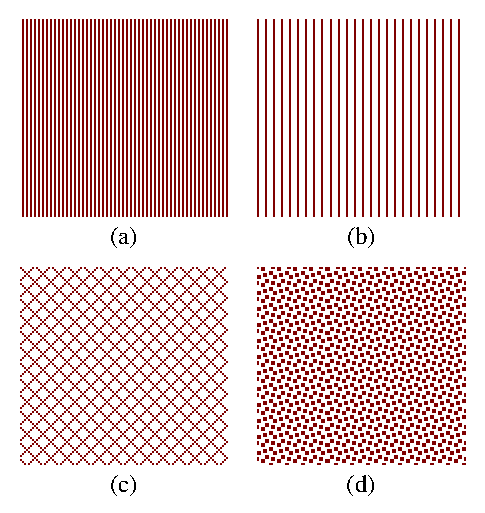
\includegraphics[width=8.3cm]{OT10000F1}
\caption{Sample figure with preferred style for labeling parts.}
\end{figure}


\begin{table}[htb]
 \centering \caption{Sample Table}
\begin{tabular}{ccc}
    \hline
    One & Two & Three \\
    \hline
    Eins & Zwei & Drei \\
    Un & Deux & Trois \\
    Jeden & Dv\v{e} & T\v{r}i \\
    \hline
   \end{tabular}
    \end{table}

No more than three figures should generally be included in the paper. Place figures as close as possible to where they
are mentioned in the text. No part of a figure should extend beyond text width, and text should not wrap around figures. Please provide permission and attribution for any trademarked or copyright images.

\section{References}
References should be cited with the \verb+\cite{}+ command.
Bracketed citation style, as opposed to superscript, is preferred
\cite{krishnan00,vantrigt97,masters93,shoop97,kalman76,craig96,steup96}.
The \texttt{osameet3.sty} style file references \texttt{cite.sty}. Comprehensive journal abbreviations are available on the Crossref web site:
\href{http://www.crossref.org/titleList/}{http://www.crossref.org/titleList/}.

\begin{thebibliography}{99} %% use BibTeX or add references manually



\bibitem{krishnan00} E. Krishnan, A. M. Shan, T. Rishi, L. A. Ajith, C. V.
Radhakrishnan, \textit{On-line Tutorial on \LaTeX{}},
``Mathematics'' (Indian \TeX{} Users Group, 2000), \\
\url{http://www.tug.org/tutorials/tugindia/chap11-scr.pdf}.

\bibitem{vantrigt97} C. van Trigt, ``Visual system-response functions and estimating reflectance,''
J. Opt. Soc. Am. A \textbf{14}, 741--755 (1997).

\bibitem{masters93} T. Masters, \emph{Practical Neural Network Recipes in C++} (Academic, 1993).

\bibitem{shoop97} B. L. Shoop, A. H. Sayles, and D. M. Litynski, ``New devices for optoelectronics: smart pixels,''
in \emph{Handbook of Fiber Optic Data Communications},
C. DeCusatis, D. Clement, E. Maass, and R. Lasky, eds. (Academic, 1997), pp. 705--758.

\bibitem{kalman76} R. E. Kalman,``Algebraic aspects of the generalized inverse of a rectangular matrix,'' in
\emph{Proceedings of Advanced Seminar on Generalized Inverse and Applications}, M. Z. Nashed, ed. (Academic, 1976), pp. 111--124.

\bibitem{craig96} R. Craig and B. Gignac, ``High-power 980-nm pump lasers,''
in \emph{Optical Fiber Communication Conference}, Vol. 2 of 1996 OSA Technical Digest Series (Optical Society of America, 1996), paper ThG1.

\bibitem{steup96} D. Steup and J. Weinzierl, ``Resonant THz-meshes,''
presented at the Fourth International Workshop on THz Electronics, Erlangen-Tennenlohe, Germany, 5--6 Sept. 1996.

\end{thebibliography}

\end{document}
